
\documentclass[10pt]{article}
\usepackage{longtable}
\usepackage{graphicx}
\usepackage{amssymb}
\usepackage[a4paper]{geometry}

 \newcommand{\qed}{\hfill \ensuremath{\Box}}
 \newenvironment{proof}{ \rm \begin{footnotesize}\noindent {\bf Proof}}{\qed \end{footnotesize}\\ \vspace{1cm} }
\cleardoublepage

\title{Documentation of  \\ReLIADiff. A C++ Software Package For Real Laplace
transform Inversion based on Algorithmic Differentiation
\footnote{Accompanying the paper in \cite{RELART}} }

\date{}


\begin{document}


\maketitle
\thispagestyle{empty}

\author{
\begin{center} LUISA D'AMORE\dag , ROSANNA CAMPAGNA\dag, VALERIA MELE\dag \\ ALMERICO MURLI\ddag \,  \

\end{center}}

{\dag\ University of Naples Federico II, Via Cintia,  Naples, Italy}


{\ddag\ CMCC -Lecce, Italy and SPACI}

\vspace{2cm}
\begin{center}
 {\large {\bf DEMOS User Guide  }}
\end{center}
\vspace{2cm}

\setlength{\parindent}{0in}


\newcommand{\itab}[1]{\hspace{0em}\rlap{#1}}
\newcommand{\tab}[1]{\hspace{.3\textwidth}\rlap{#1}}

\newpage
\setcounter{page}{1}
\tableofcontents

\newpage

%-------------------------------------------------------------------------------------------------------------------------
\section{Introduction}\label{intro}

In the directory {\tt C++\_files/demos-Linux\_g++} users find demos to compile and execute on a Linux system with a g++ compiler installed.\\


\begin{figure}[!h]
\begin{flushright}
%[scale=0.6]
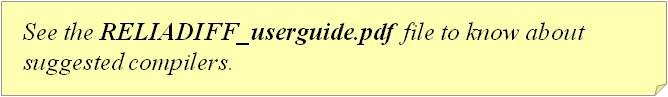
\includegraphics[scale=0.8]{Immagine1}
\end{flushright}
\end{figure}



Demos use RELIADIFF
\begin{enumerate}
	\item On a function of the Laplace Transform/Inverse database (in\\{\tt DEMO1-Functions\_From\_DATABASE})
		      \begin{itemize}
		      \item User may give different arguments in the provided shell scripts.
		      \item Demo generates a file with results.
		      \end{itemize}
	\item On a Laplace Transform, to be defined in the demo with its Inverse (in {\tt DEMO2-Function\_To\_Give})
		      \begin{itemize}
		      \item User may change the Transform/Inverse definition (and the related parameter szero in the main program) \underline{before} to compile to test RELIADIFF on his own.
		      \item Demo generates a file with results.
		      \end{itemize}
\end{enumerate}

\section{Content of DEMOS directory}
The directory {\tt C++\_files/demos-Linux\_g++} contains three directories and two files:
\begin{itemize}
	  \item DEMO1\textendash Functions\textendash From\textendash DATABASE

\begin{figure}[!h]
\begin{flushright}

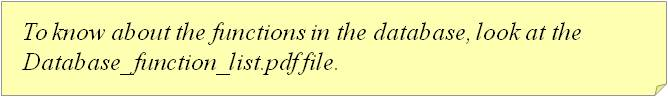
\includegraphics[scale=0.8]{Immagine2}

\end{flushright}
\end{figure}

	  \item DEMO2\textendash Function\textendash To\textendash Give

\begin{figure}[!h]
\begin{flushright}

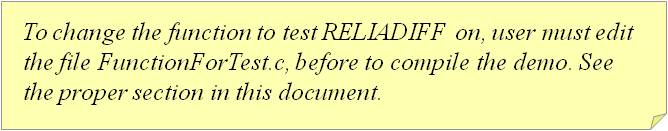
\includegraphics[scale=0.8]{Immagine3}

\end{flushright}
\end{figure}

		    \begin{itemize}
		      \item The demo will generate a file with results for the defined function.
		    \end{itemize}
	  \item utility: files containing utility routines needed to execute functions in the database and the demos.
	  Here are also functions to print in a file the role of the \emph{flag}, \emph{Ncalc} and \emph{Nopt} variables returned by RELIADIFF.

\begin{figure}[!h]
\begin{flushright}

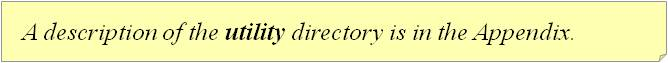
\includegraphics[scale=0.8]{Immagine4}
\end{flushright}
\end{figure}

	  \item gsl\textendash 1.15.tar.gz: a compressed file containing the installation files for the GNU Scientific Library (GSL), that user could need to install.
	  \item Makefile\_gsl: makefile installing  the GSL locally, if it is needed.

\begin{figure}[!h]
\begin{flushright}

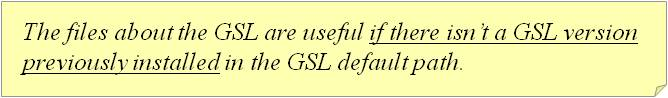
\includegraphics[scale=0.8]{Immagine5}

\end{flushright}
\end{figure}

\end{itemize}



\section{DEMO 1}
\subsection{Purpose}
In the directory \textbf{{\tt DEMO1-Function\_From\_DATABASE}} users find files to build a demo\textendash program driving tests of RELIADIFF routine on the functions in the database.

\begin{figure}[!h]
\begin{flushright}

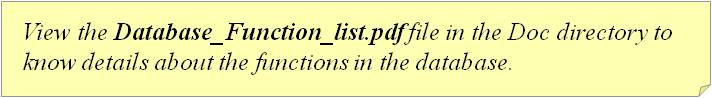
\includegraphics[scale=0.8]{Immagine6}

\end{flushright}
\end{figure}

\subsection{Description}
This main program:
      \begin{itemize}
      \item obtains the needed parameter from the user
	\item sets the abscissa of convergence depending on the function chosen by the user
	\item sets the \emph{szero} parameter as needed by the function chosen by the user
		  \begin{itemize}
		  \item \emph{szero=1} if the Transform has a singularity at zero
		  \end{itemize}

      \item calls RELIADIFF routine for each evaluation point required by the user
      \item compare the results with the known inverse values
      \item prints the output in a txt file named with the number of the function
      \end{itemize}

The user can choose how many functions and which ones to use.

\begin{figure}[!h]
\begin{flushright}
%[scale=0.6]
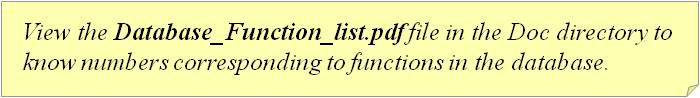
\includegraphics[scale=0.8]{Immagine7}
\end{flushright}
\end{figure}

\subsection{Content of directory}

The directory contains:
      \begin{itemize}
      \item \textbf{TEST\_ON\_DATABASE.c}: the main program
      \item \textbf{Makefile}: to compile the demo with a GNU Scientific Library (GSL) already installed (as root in the default path).
		    \begin{itemize}
		      \item The command {\tt make} compiles the c file linking the needed, to obtain the executable file {\tt test\_on\_database}
		    \item The command {\tt make clean} deletes executable file, the txt files in the directory and the created libraries
		    \end{itemize}
      \item \textbf{database}: files needed to generate a library of 89 functions that authors used to test  RELIADIFF.

\begin{figure}[!h]
\begin{flushright}

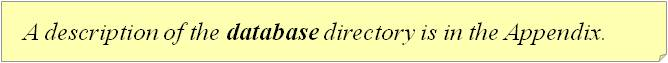
\includegraphics[scale=0.8]{Immagine8}

\end{flushright}
\end{figure}

      \item \textbf{scripts}: 6 shell scripts running the program with different kinds of input.
		      \begin{itemize}
		      \item \textbf{TESTONE\_defaultParameters.sh}:	a shell script running the program passing no arguments (user shall explicitly choose a function at runtime, giving the corresponding number when required)

		      \item \textbf{TESTONE\_givenPoints.sh}:	a shell script running the program on a single function with all default parameters but explicitly giving some evaluation points (user shall explicitly choose a function at runtime, giving the corresponding number when required)

		      \item \textbf{TESTONE\_tol\textendash 3.sh}:	a shell script running the program on a single function providing the required accuracy (\emph{tol=$1^{-3}$}) and giving a range for the evaluation points (user shall explicitly choose a function at runtime, giving the corresponding number when required)

		      \item \textbf{TEST\_10\_tol\textendash 4.sh}:	a shell script running the program with \emph{tol=$1^{-4}$}, on 10 functions from database (the user shall explicitly choose the functions at runtime, giving a number a time when required)

		      \item \textbf{TESTALL\_tol\textendash 4.sh}:	a shell script running the program with \emph{tol=$1^{-4}$}, on all the functions in the provided database, giving a range for the evaluation points and printing all the used coefficients for each evaluation point.

		      \item \textbf{TESTALL\_defaultParameters.sh}:	a shell script running the program on all the functions in the database without any other argument
		      \end{itemize}
      \end{itemize}



The directory contains also:
    \begin{itemize}
    \item \textbf{Makefile\_gslloc}: just to compile the demo with a GNU Scientific Library (GSL) installed locally, if user does not already have one installed in the default path.
	  \begin{itemize}
	  \item command {\tt make -f Makefile\_gslloc} compiles the c file linking the libraries, to obtain the executable file {\tt test\_on\_database}
	  \end{itemize}
    \end{itemize}


\subsection{How to compile}

\subsubsection{GSL already installed in /usr/local/}

By default, the GSL is installed in
\begin{itemize}
 \item {\tt /usr/local/bin},
 \item {\tt /usr/local/man},
 \item {\tt /usr/local/lib},
 \item {\tt /usr/local/include},
 \item ...
\end{itemize}
That is in {\tt /usr/local/}. So, if you previously installed the GSL without changing path:
\begin{enumerate}
 \item Enter the directory {\tt demos-Linux\_g++/DEMO1-Functions\_From\_DATABASE}
 \item Type the command {\tt make}
\end{enumerate}

\subsubsection{GSL already installed in a different path}

When installing GSL user can specify an installation prefix other than `{\tt /usr/local}' by giving {\tt configure} the
option `{\tt --prefix=PATH}'. So, if you previously installed the GSL changing path:
\begin{enumerate}
 \item Find the path of the GSL: {\tt /yourpath/} (example: {\tt /usr/}).
\item Enter the directory {\tt demos-Linux\_g++/DEMO1-Functions\_From\_DATABASE}.
\item Open the file {\tt Makefile}.
\item Edit only the path for the \emph{gsllib} variable (as shown in the figure \ref{fig:gsl1}).

\begin{figure}[!h]
\begin{center}
%[scale=0.6]
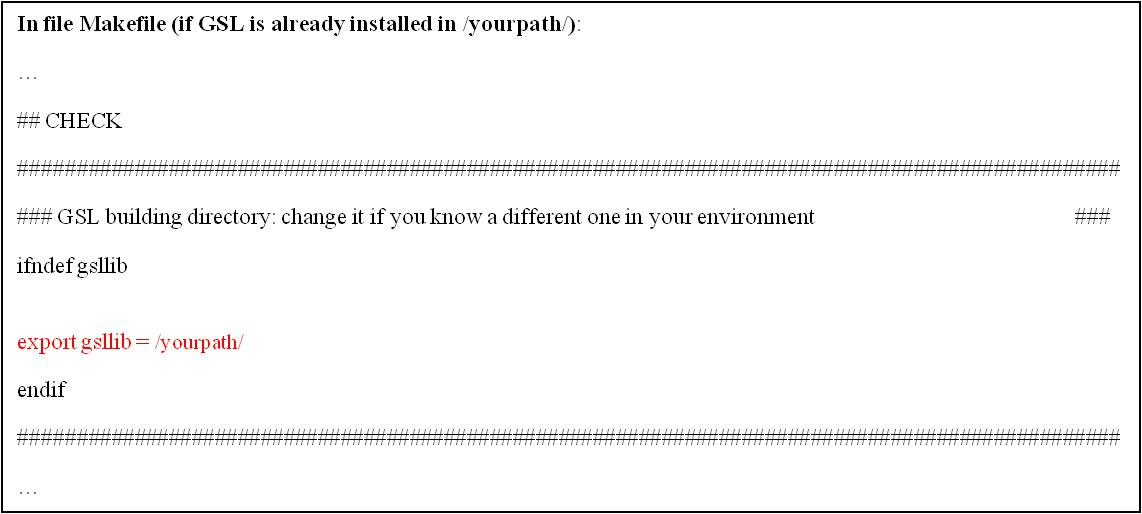
\includegraphics[scale=0.6]{Immagine9}
\caption{\label{fig:gsl1}In red the path to change in the Makefile.}
\end{center}
\end{figure}


\item Type the command make.
\end{enumerate}




\subsubsection{GSL not installed}
\begin{enumerate}
 \item Install the GSL locally (in the {\tt C++\_files/demos-Linux\_g++/GSL} directory), that is
	    \begin{enumerate}
	    \item Enter the {\tt demos-Linux\_g++} directory
	    \item Type the command {\tt make -f Makefile\_gsl}
	    \end{enumerate}
 \item Enter the directory {\tt demos-Linux\_g++/DEMO1-Functions\_From\_DATABASE}
 \item Type the command {\tt make -f Makefile\_gslloc}
\end{enumerate}

\subsection{How to execute}

After compiling, with the makefile, in this directory there will be an executable file named {\tt test\_on\_database}.\\
To execute it, user should only provide it the arguments he/she wants, as described at the previous point:\\

{\tt ./test\_on\_database [ordered list of arguments]}\\

or he/she may use one of the provided scripts, described at the beginning of this section.


\subsection{Arguments}

The user may execute {\tt test\_on\_database} with 6 kinds of INPUT:
\begin{enumerate}
 \item \textbf{none argument}
 \item \textbf{one argument}
 \item \textbf{two arguments}
 \item \textbf{three arguments}
 \item \textbf{four arguments}
 \item \textbf{more than seven arguments}
\end{enumerate}

Where:
\begin{enumerate}
	\item \textbf{none argument}: The driver uses all default values:\\
	      \itab{\emph{tol}} \tab{required accuracy}\\
	      \itab{\emph{ntf= 1}} \tab{number of functions testing RELIADIFF with}\\
	      \itab{\emph{nmax= 2000}} \tab{maximum number of series coefficients}\\
	      \itab{\emph{pcoeff= 0}} \tab{do not print coefficients}\\
	      \itab{\emph{x= 1, 5, 10, 15}} \tab{evaluation points}

	\item \textbf{1 argument}: \emph{tol} (if it is a string "n" it is posed equal to the default value).\\ The driver will use other default values:\\
	      \itab{\emph{ntf= 1}}\\
	      \itab{\emph{nmax= 2000}}\\
	      \itab{\emph{pcoeff= 0}}\\
	      \itab{\emph{x= 1, 5, 10, 15}}

	\item \textbf{2 arguments}: \emph{tol}, \emph{ntf} (if one is a string "n" it is posed equal to the default value; if \emph{ntf} is the string "a" it is posed equal to the total number of functions in the database). \\The driver will use other default values:\\
	      \itab{\emph{nmax=2000}}\\
	      \itab{\emph{pcoeff= 0}}\\
	      \itab{\emph{x= 1, 5, 10, 15}}

	\item \textbf{3 arguments}: \emph{tol}, \emph{ntf}, \emph{nmax} (if one is a string "n" it is posed equal to the default value; if \emph{ntf} is the string "a" it is posed equal to the total number of functions in the database). \\The driver will use other default values:\\
	      \itab{\emph{pcoeff= 0}}\\
	      \itab{\emph{x= 1, 5, 10, 15}}

	\item \textbf{4 arguments}: \emph{tol}, \emph{ntf}, \emph{nmax}, \emph{pcoeff} (if one is a string "n" it is posed equal to the default value; if \emph{ntf} is the string "a" it is posed equal to the total number of functions in the database). \\The driver will use other default values.\\
		\itab{\emph{x= 1, 5, 10, 15}}

	\item \textbf{$>7$ arguments}: \emph{tol}, \emph{ntf}, \emph{nmax}, \emph{pcoeff} (if one is a string "n" it is posed equal to the default value; if \emph{ntf} is the string "a" it is posed equal to the total number of functions in the database); the  5\textendash th argument \emph{range} should be 0 or greater:
	\begin{itemize}
	 \item IF \emph{range$>$0} the inverse functions are computed on a set of equispaced points belonging to the interval [a,b] with step size "step". In this case:\\
		  \tab{6\textendash th argument: \emph{a},}\\
		  \tab{7\textendash th argument: \emph{b},}\\
		  \tab{8\textendash th argument: \emph{step}}\\
	\item IF \emph{range=0} the inverse functions are computed on a given set of values. In this case:\\
		  \tab{6\textendash th argument: \emph{dim}, is the number of evaluation points};\\
		  \tab{7\textendash th until to (6+dim)\textendash th argument: \emph{the evaluation points}.}
	\end{itemize}



\end{enumerate}


\subsubsection{Return value}
\emph{Return value}: 0 if the program runs without any problem


\section{DEMO 2}

\subsection{Purpose}
In the directory \textbf{{\tt DEMO2-Function\_To\_Give}} users find files to build a demo\textendash main program driving tests of RELIADIFF routine on a provided Laplace Transform with its Inverse provided too.
\subsection{Description}

This main program:
\begin{itemize}
    \item obtains the needed parameter from the user
    \item sets the \emph{szero} parameter as needed by the function
	    \begin{itemize}
	      \item \emph{szero} should be 1 if the Transform has a singularity at zero
	    \end{itemize}
    \item calls RELIADIFF routine
    \item compares the result with the known inverse value
    \item prints the output in a txt file named {\tt output\_demo2.txt}

\end{itemize}

\subsection{Content of directory}

The directory contains 4 files and a directory:
\begin{itemize}
 \item \textbf{TEST\_FunctionToGive.c}: main program

 \item \textbf{FunctionForTest.c}: containing the definition of the function to invert and of the true inverse to compare to (the user should modify this function in this file as well as he needs).

\begin{figure}[!h]
\begin{flushright}

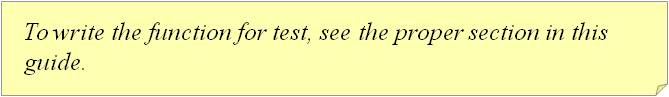
\includegraphics[scale=0.8]{Immagine10}

\end{flushright}
\end{figure}


 \item \textbf{Makefile}: compiling the demo with a GNU Scientific Library (GSL) installed as root in the default path.
	    \begin{itemize}
	    \item The command {\tt make} compiles the c file linking the libraries, to obtain the executable file {\tt test\_functiontogive}
	    \item The command {\tt make clean} deletes executable file, the txt files in the directory and the created libraries
	    \end{itemize}
 \item \textbf{Makefile\_gslloc}: compiling the demo with a GNU Scientific Library (GSL) installed locally.
	    \begin{itemize}
	    \item The command {\tt make –f Makefile\_gslloc} compiles the c file linking the libraries, to obtain the executable file file {\tt test\_functiontogive}
	    \end{itemize}
 \item \textbf{scripts}:	6 shell scripts to run the program with different kinds of input.
	    \begin{itemize}

	    \item \textbf{TEST\_default.sh}: a shell script running the program with no argument

	    \item \textbf{TEST\_givenpoints.sh}: a shell script running the program providing explicitly some evaluation points

	    \item  \textbf{TEST\_somedefaultvalues.sh}:	a shell script running the program with some default values in arguments
	    \end{itemize}
 \end{itemize}





\subsection{How to write the function to test}

User should write the Transform, named \textbf{fzE}, and its Inverse function, named \textbf{gzE}, in the file {\tt TEST\_FunctionForTest.c}, replacing those given as example.\\
\textbf{fzE} must require in input:
 \begin{itemize}
 \item \emph{z:} ({\tt TADIFF}) double precision: the evaluation point of the Transform

 \begin{figure}[!h]
\begin{flushright}

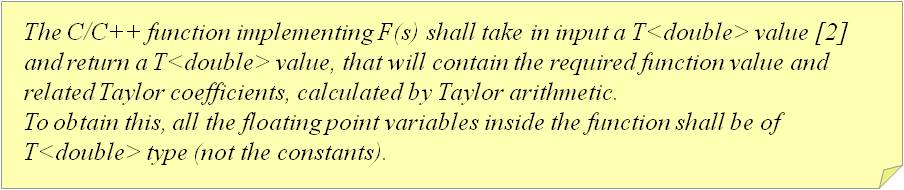
\includegraphics[scale=0.8]{Immagine11}

\end{flushright}
\end{figure}

 \end{itemize}
and returns:
 \begin{itemize}
 \item ({\tt TADIFF}) double precision: the evaluation of the Transform at \emph{z:}
 \end{itemize}

\textbf{gzE} must require in input:
 \begin{itemize}
 \item \emph{t}: double precision: the evaluation point of the Inverse function
 \end{itemize}
and returns:
 \begin{itemize}
 \item double precision: the evaluation of the Inverse function at \emph{t}
 \end{itemize}

\subsection{How to compile}

\subsubsection{GSL already installed in /usr/local/}

By default, the GSL is installed in
\begin{itemize}
 \item {\tt /usr/local/bin},
 \item {\tt /usr/local/man},
 \item {\tt /usr/local/lib},
 \item {\tt /usr/local/include},
 \item ...
\end{itemize}
That is in {\tt /usr/local/}. So, if you previously installed the GSL without changing path:
\begin{enumerate}
 \item Enter the directory {\tt demos-Linux\_g++/DEMO2-Function\_To\_Give}
 \item Type the command {\tt make}
\end{enumerate}


\subsubsection{GSL already installed in a different path}

When installing GSL user can specify an installation prefix other than `{\tt /usr/local}' by giving `{\tt configure}' the
option `{\tt --prefix=PATH}'. So, if you previously installed the GSL changing path:
\begin{enumerate}
 \item Find the path of the GSL: {\tt /yourpath/} (example: {\tt /usr/}).
\item Enter the directory {\tt demos-Linux\_g++/DEMO2\textendash Function\_To\_Give}.
\item Open the file Makefile.
\item Edit only the path for the \emph{gsllib} variable (as shown in the figure \ref{fig:gsl2}).

\begin{figure}[!h]
\begin{center}
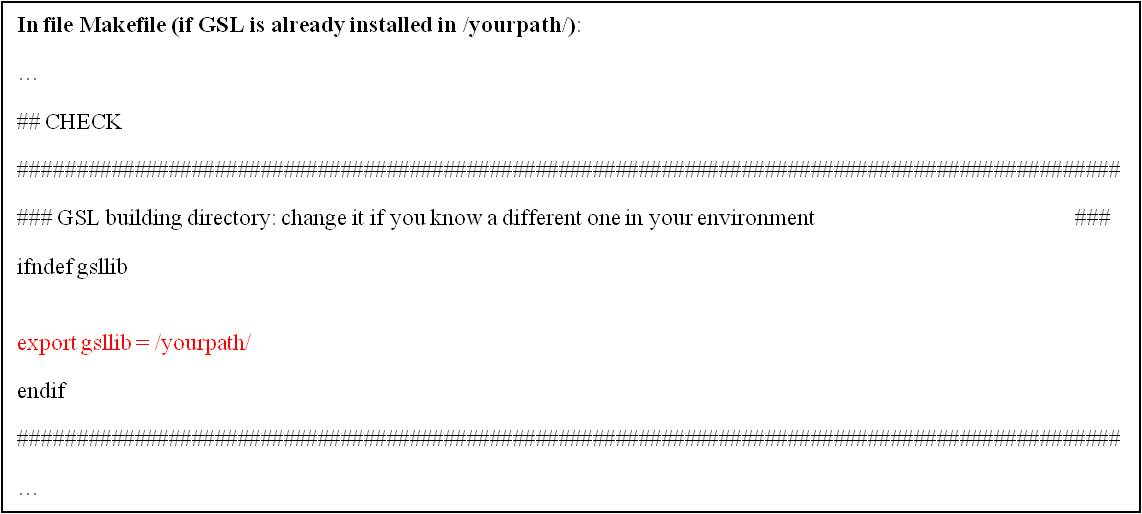
\includegraphics[scale=0.6]{Immagine12}
\caption{\label{fig:gsl2}In red the path to change in the Makefile.}
\end{center}
\end{figure}

\item Type the command {\tt make}.
\end{enumerate}


\subsubsection{GSL not installed}
\begin{enumerate}
 \item Install the GSL locally (in the {\tt C++\_files/demos-Linux\_g++/GSL} directory), that is
	  \begin{enumerate}
	  \item Enter the {\tt demos-Linux\_g++} directory
	  \item Type the command {\tt make -f Makefile\_gsl}
	  \end{enumerate}
 \item Enter the directory {\tt demos-Linux\_g++/DEMO2-Function\_To\_Give}
 \item Type the command {\tt make -f Makefile\_gslloc}
\end{enumerate}

\subsection{How to execute}
After compiling, with the makefile, in this directory there will be an executable file named {\tt test\_functiontogive}.\\
To execute it, user should only provide it the arguments he/she wants, as described at the previous point:\\

{\tt ./test\_functiontogive [ordered list of arguments]}\\

or he/she may use one of the provided scripts, described at the beginning of this section.


\subsection{Arguments}
The user may execute {\tt test\_functiontogive} with 7 kinds of INPUT:
\begin{enumerate}
\item \textbf{none argument}
 \item \textbf{one argument}
 \item \textbf{two arguments}
 \item \textbf{three arguments}
 \item \textbf{four arguments}
 \item \textbf{five arguments}
 \item \textbf{more than seven arguments}
\end{enumerate}

Where:
\begin{enumerate}
	  \item \textbf{none argument}: The driver uses all default values:\\
		  \itab{\emph{tol= $10^{-3}$}} \tab{required accuracy}\\
		  \itab{\emph{sigma0= 1}} \tab{convergence abscissa for the Transform}\\
		  \itab{\emph{nmax= 2000}} \tab{maximum number of series coefficients}\\
		  \itab{\emph{pcoeff= 0}} \tab{do not print coefficients}\\
		  \itab{\emph{szero= 0}} \tab{the Laplace transform has not a singularity at zero}\\
		  \itab{\emph{x= 1, 5, 10, 15}} \tab{evaluation points}

	  \item \textbf{1 argument}: \emph{tol} (if it is a string "n" it is posed equal to the default value). \\The driver will use other default values:\\
		  \itab{\emph{sigma0= 1}}\\
		  \itab{\emph{nmax= 2000}}\\
		  \itab{\emph{pcoeff= 0}}\\
		  \itab{\emph{szero= 0}}\\
		  \itab{\emph{x= 1, 5, 10, 15}}

	  \item \textbf{2 arguments}: \emph{tol}, \emph{sigma0} (if one is a string "n" it is posed equal to the default value). \\The driver will use other default values:\\
		\itab{\emph{nmax=2000}}\\
		\itab{\emph{pcoeff= 0}}\\
		\itab{\emph{szero= 0}}\\
		\itab{\emph{x= 1, 5, 10, 15}}

	  \item \textbf{3 arguments}: \emph{tol}, \emph{sigma0}, \emph{nmax} (if one is a string "n" it is posed equal to the default value). \\The driver will use other default values:\\
		\itab{\emph{pcoeff= 0}}\\
		\itab{\emph{szero= 0}}\\
		\itab{\emph{x= 1, 5, 10, 15}}

	  \item \textbf{4 arguments}: \emph{tol}, \emph{sigma0}, \emph{nmax}, \emph{pcoeff} (if one is a string "n" it is posed equal to the default value). \\The driver will use other default values:\\
		\itab{\emph{szero= 0}}\\
		\itab{\emph{x= 1, 5, 10, 15}}

	  \item \textbf{5 arguments}: \emph{tol}, \emph{sigma0}, \emph{nmax}, \emph{pcoeff}, \emph{szero} (if one is a string "n" it is posed equal to the default value). \\The driver will use other default values:\\
		\itab{\emph{x= 1, 5, 10, 15}}

	  \item \textbf{$>8$ arguments}: \emph{tol}, \emph{sigma0}, \emph{nmax}, \emph{pcoeff}, \emph{szero} (if one is the string "n" it is posed equal to the default value); the 6\textendash th argument \emph{range},  should be 0 or greater.
	  \begin{itemize}
	   \item  IF \emph{range$>$0} the inverse functions are computed on a set of equispaced points belonging to the interval [a,b] with step size "step". In this case:\\
			  \tab{7\textendash th argument: \emph{a},}\\
			  \tab{8\textendash th argument: \emph{b},}\\
			  \tab{9\textendash th argument: \emph{step}}\\
	    \item IF \emph{range=0} the inverse functions  are computed on a given set of values. In this case:\\
			  \tab{7\textendash th argument: \emph{dim}, is the number of evaluation points}\\
			  \tab{8\textendash th until to  (7+dim)\textendash th argument: \emph{the evaluation points}.}
	  \end{itemize}



\end{enumerate}


\subsubsection{Return value}
\emph{Return value}: 0 if the program runs without any problem



\section{Appendix}
In this section we will describe two other directories in the package.

\subsection{Utility}
\subsubsection{Purpose}
In this directory users find some utility tools.

\subsubsection{Description}

There are some function computing
\begin{itemize}
 \item The integer power of a real number (in the {\tt TADIFF} definition)
 \item The Laguerre polynomial
 \item The Hermite polynomial
\end{itemize}

There are also two routines writing on a file the explanation of the role of the \emph{flag}, \emph{Ncalc} and \emph{Nopt} variables returned by RELIADIFF.

\subsubsection{Content}

The directory {\tt C++\_files/demos-Linux\_g++/utility} contains 4 files which are:
\begin{itemize}
	\item \textbf{Util.c}	containing a library of functions needed by the functions of the database and useful to write a function to test the RELIADIFF routine. There are also routines writing the on a file the explanation of the role of the \emph{flag}, \emph{Ncalc} and \emph{Nopt} variables returned by RELIADIFF.
	\item \textbf{Util.h}	containing some header inclusions, and the prototypes of the functions defined in {\tt Util.c}. It includes RELIADIFF.h and the GSL headers
	\item Two makefiles :
		\begin{itemize}
		\item \textbf{Makefile} compiling the database library with GSL installed in the default path.
		      \begin{itemize}
		      \item The command {\tt make} creates the library {\tt libutil.a}
		      \item The command {\tt make clean} deletes the {\tt libutil.a} file
		      \end{itemize}
		\item \textbf{Makefile\_gslloc} compiling the database library with a locally installed GSL.
		      \begin{itemize}
		      \item The command {\tt make –f Makefile\_gslloc} creates the library {\tt libutil.a}
		      \end{itemize}
		\end{itemize}
\end{itemize}

 \begin{figure}[!h]
\begin{flushright}

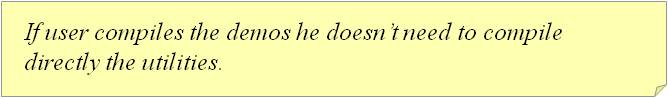
\includegraphics[scale=0.8]{Immagine13}
\end{flushright}
\end{figure}

\subsubsection{Specification of Utility functions}
There are 5 functions:

\paragraph{Integer power of a {\tt TADIFF}\textendash double precision variable} \ \\

{\tt T<double> pow\_int\_T(T<double> a, int n)}\\

\begin{longtable}{ll}
\texttt{a}: &({\tt TADIFF}) double precision: the base\\
\texttt{n}: &integer: the exponent\\
\emph{return value}: &({\tt TADIFF}) double precision: the n\textendash power of a\\
 \end{longtable}


\paragraph{Computation of the Laguerre Polynomial in \texttt{x} of degree \texttt{K}}\ \\

{\tt double Laguerre(int K, double x)}\\

\begin{longtable}{ll}
\texttt{K}: &integer: degree of the Hermite polynomial to calculate\\
\texttt{x}: &double precision: point of evaluation\\
\emph{return value}: &double precision: Hermite polynomial at \texttt{x}\\
 \end{longtable}


\paragraph{Computation of the Hermite Polynomial in \texttt{x} of degree \texttt{K}}\ \\

{\tt double Hermite(int K, double x)}\\
\begin{longtable}{ll}
\texttt{K}: &integer: degree of the Hermite polynomial to calculate\\
\texttt{x}: &double precision: point of evaluation\\
\emph{return value}: &double precision: Hermite polynomial at \texttt{x}\\
 \end{longtable}

\paragraph{Printing in file the diagnostics parameters interpretation: flag}\ \\

{\tt void print\_flags\_file(FILE *fp)}\\
\begin{longtable}{ll}
\texttt{fp}: &file handler: handler of the file where to write the flag meaning\\&in RELIADIFF\\
 \end{longtable}

\paragraph{Printing in file the diagnostics parameters interpretation: ncalc and nopt}\ \\

{\tt void print\_N\_file(FILE *fp, int nmax)}\\
\begin{longtable}{ll}
\texttt{fp}: &file handler: handler of the file where to write Nopt/Ncalc meaning\\&in RELIADIFF\\
\texttt{nmax}: &integer: required maximum number of Taylor coefficients to calculate\\&in RELIADIFF\\
 \end{longtable}




\subsection{DEMO1\textendash Function\_From\_DATABASE/Database}

\subsubsection{Purpose}
In this directory, users find a library of Laplace Transforms and of the related Inverse functions.
The database contains 89 functions.


\subsubsection{Content}
The directory database contains 4 files which are:
\begin{itemize}
	\item \textbf{dbLaplace.c}:	containing the Laplace Transforms
	\item \textbf{dbInvLaplace.c}:	containing the Inverse Laplace Transforms
	\item \textbf{dbL.h}:	containing the prototypes of functions defined in {\tt dbLaplace.c} and {\tt dbInvLaplace.c}. It includes {\tt Util.h}.
	\item Two makefiles :
	    \begin{itemize}
	    \item \textbf{Makefile} compiling the database library with GSL installed in the default path.
		    \begin{itemize}
		    \item The command {\tt make} creates the library {\tt libdatabase.a}
		    \item The command {\tt make clean} deletes the {\tt libdatabase.a} file
		    \end{itemize}
	    \item \textbf{Makefile\_gslloc} compiling the database library with a locally installed GSL.
		    \begin{itemize}
		    \item The command {\tt make –f Makefile\_gslloc} creates the library {\tt libdatabase.a}
		    \end{itemize}
	    \end{itemize}
\end{itemize}

 \begin{figure}[!h]
\begin{flushright}
%[scale=0.6]
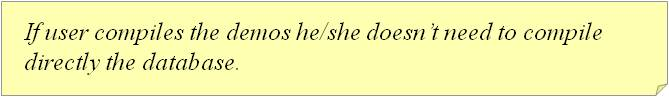
\includegraphics[scale=0.8]{Immagine14}
\end{flushright}
\end{figure}


\subsubsection{Specification of Database functions}

Each Transform function is of the kind\\
{\tt T<double>  fzXX(T<double> z)} \\
where “XX” is the number of the function in the database.\\

Each Inverse function is of the kind\\
{\tt double gzXX(double)}\\
where “XX” is the number of the function in the database.\\

 \begin{figure}[!h]
\begin{flushright}

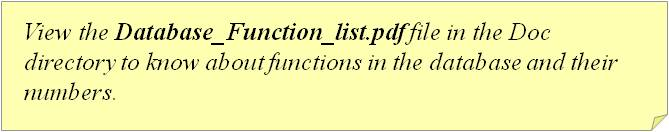
\includegraphics[scale=0.8]{Immagine15}
\end{flushright}
\end{figure}

\begin{figure}[!h]
\begin{flushright}

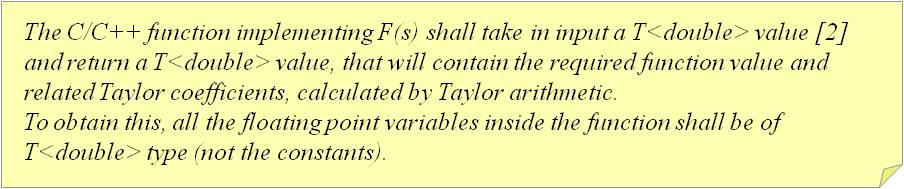
\includegraphics[scale=0.8]{Immagine16}
\end{flushright}
\end{figure}

\newpage

\begin{thebibliography}{10}
\bibitem{RELART} A. Murli, L. D'Amore, V. Mele, R. Campagna, \emph{ReLIADiff. A C++ Software Package For Real Laplace
transform Inversion based on Algorithmic Differentiation}, ACM Transactions on Mathematical Software,
0, 0, Article 0 ( 0000), 20 pages.

\bibitem{TADIFF} C. Bendtsen, O. Stauning, \emph{ Tadiff, a flexible C++ package for Automatic Differentiation using Taylor series expansion}, technical report IMM-REP-1997-07, Department of Mathematical Modelling, Technical University of Denmark, 2800 Lyngby, Denmark, 1997.

\end{thebibliography}

\end{document}
